
\documentclass[preprint,12pt]{elsarticle}

\usepackage[spanish]{babel}
\usepackage{amssymb}
\usepackage{graphicx}
\usepackage{lineno}
\usepackage[utf8]{inputenc}
\usepackage{url}
\usepackage{natbib} 
\usepackage{amsmath} 
\usepackage{amssymb} 
\usepackage{float}

\begin{document}
	
	\begin{frontmatter} 

		\title{\huge INSTALACIÓN DE UNA INSTANCIA DE MICROSOFT SQL SERVER INFORME DE LABORATORIO 07 }
		
		\author{Pacora Silva Jorge Carlos         	(2013000725)} 
		\address{Escuela Profesional de Ingeniería de Sistemas}
		\address{Universidad Privada de Tacna}
		\address{Tacna, Perú}
	\end{frontmatter}



\section{INFORMACIÓN GENERAL} 

\subsection {\textbf{Objetivos}}
\begin{itemize}
	\item Instalación de SQL Server en Docker
	\item Usar docker con SQL Server Management Studio
\end{itemize}

\subsection {\textbf{Equipos, materiales, programas y recursos utilizados}}
\begin{itemize}
	\item Computadora con sistema operativo Windows XP, Vista, Windows 7, Windows 8 y/o Windows 8.1.
	\item Docker Desktop
	\item Microsoft SQL Server Management Studio
\end{itemize}


\section{Marco Teórico}


\subsection {\textbf{Docker}}
Docker es un proyecto de código abierto que automatiza el despliegue de aplicaciones dentro de contenedores de software, proporcionando una capa adicional de abstracción y automatización de virtualización de aplicaciones en múltiples sistemas operativos.
\subsection {\textbf{Contenedores}}
Un contenedor es más ligero, ya que mientras que a una máquina virtual necesitas instalarle un sistema operativo para funcionar, un contenedor de Docker funciona utilizando el sistema operativo que tiene la máquina en la que se ejecuta el contenedor.
\subsection{\textbf{SQL Server Management Studio}}
SQL Server Management Studio es una aplicación de software lanzada por primera vez con Microsoft SQL Server 2005 que se usa para configurar, administrar y administrar todos los componentes dentro de Microsoft SQL Server. Es el sucesor del Enterprise Manager en SQL 2000 o antes.


\section{PROCEDIMIENTO}

\subsubsection{\textbf{Paso 1: Verificar la disponibilidad de Docker}}
\begin{figure}[H]
	\begin{center}
		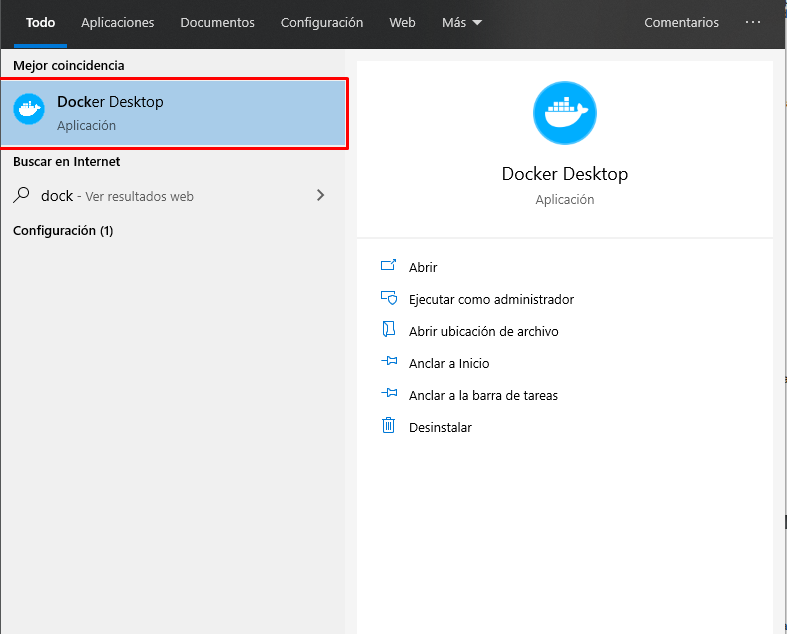
\includegraphics[width=12cm]{./IMAGENES/foto1} 
		\caption{Vizualizar Docker Setup}
	\end{center}
\end{figure}
\begin{figure}[H]
	\begin{center}
		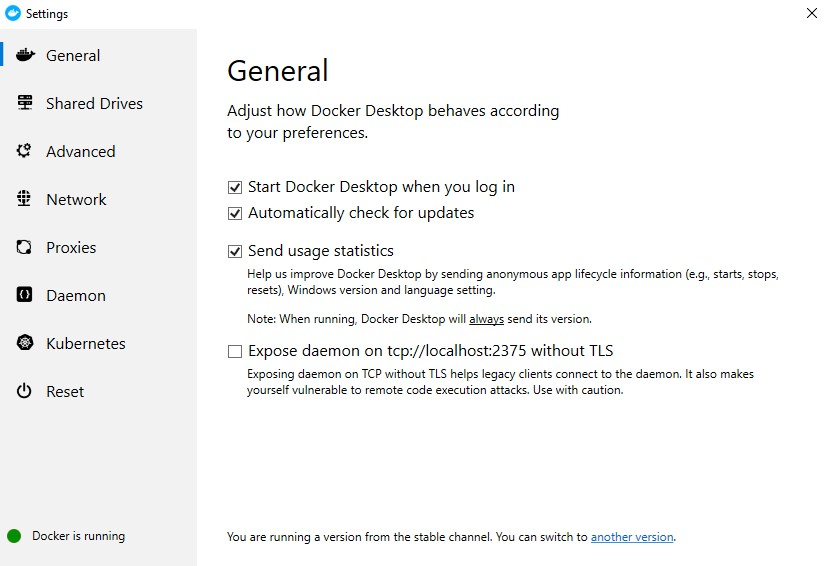
\includegraphics[width=12cm]{./IMAGENES/foto4} 
		\caption{Mostrando el menu de docker}
	\end{center}
\end{figure}

\subsubsection{\textbf{Paso 2: Usando los Comandos en Docker}}

\begin{figure}[H]
	\begin{center}
		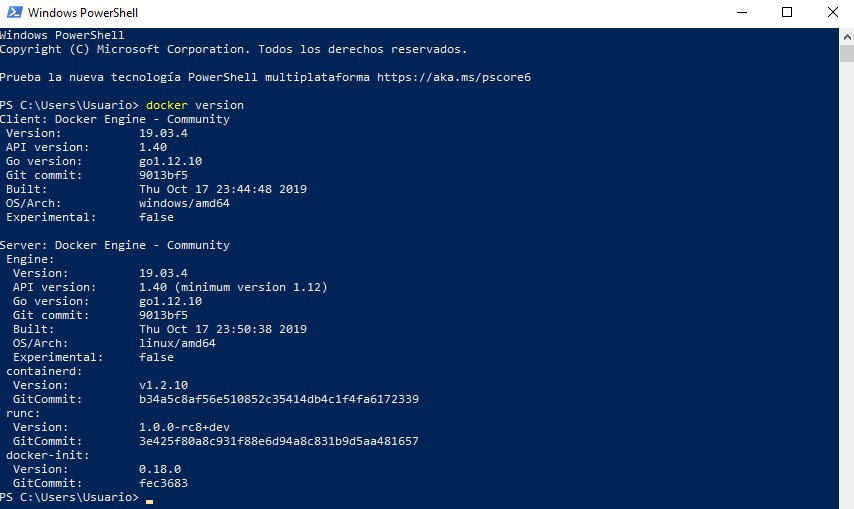
\includegraphics[width=12cm]{./IMAGENES/foto5} 
		\caption{Docker version que nos mostrara algunas especificaciones}
	\end{center}
\end{figure}


\begin{figure}[H]
	\begin{center}
		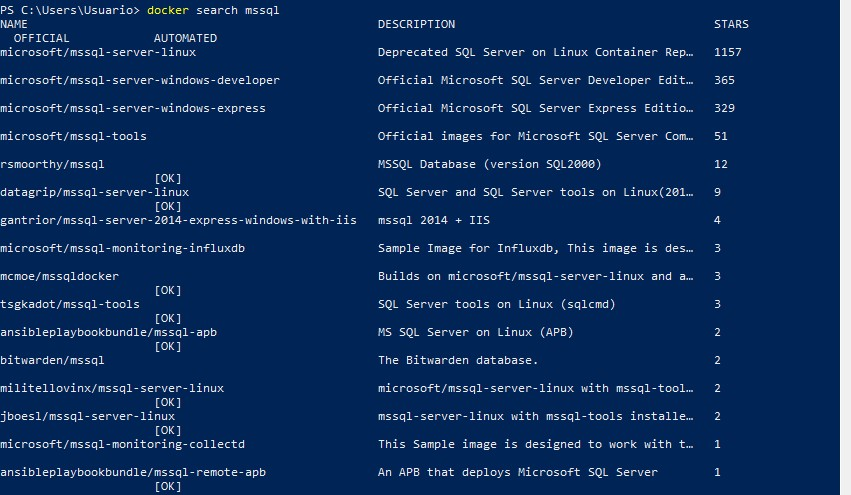
\includegraphics[width=12cm]{./IMAGENES/foto6} 
		\caption{Buscando la iso de MSSQL}
	\end{center}
\end{figure}

\begin{figure}[H]
	\begin{center}
		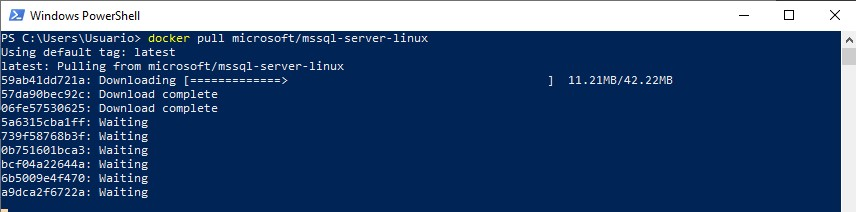
\includegraphics[width=12cm]{./IMAGENES/foto7} 
		\caption{Descargando la ISO}
	\end{center}
\end{figure}
\begin{figure}[H]
	\begin{center}
		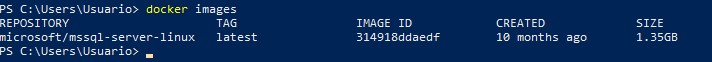
\includegraphics[width=12cm]{./IMAGENES/foto9} 
		\caption{Listamos las "images" descargadas}
	\end{center}
\end{figure}

\begin{figure}[H]
	\begin{center}
		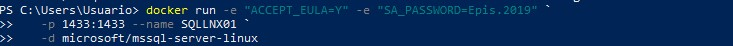
\includegraphics[width=12cm]{./IMAGENES/foto10} 
		\caption{instalamos MSSQL-Server}
	\end{center}
\end{figure}

\begin{figure}[H]
	\begin{center}
		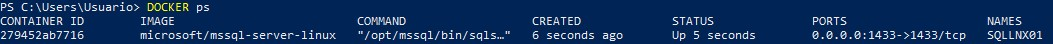
\includegraphics[width=12cm]{./IMAGENES/foto11} 
		\caption{Verificamos la instalacion}
	\end{center}
\end{figure}

\subsubsection{\textbf{Paso 3: Microsoft SQL Server Management Studio}}
\begin{figure}[H]
	\begin{center}
		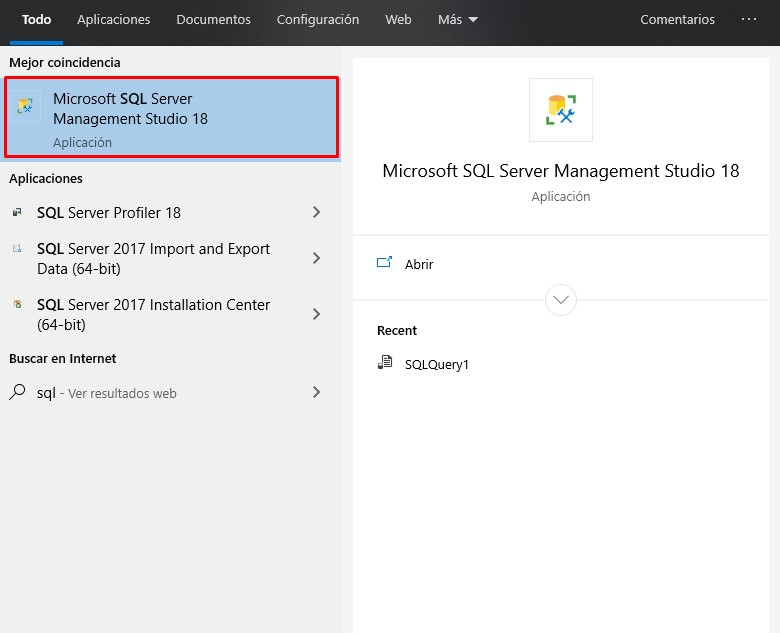
\includegraphics[width=12cm]{./IMAGENES/foto12} 
		\caption{Ingresamos a Management Studio}
	\end{center}
\end{figure}

\begin{figure}[H]
	\begin{center}
		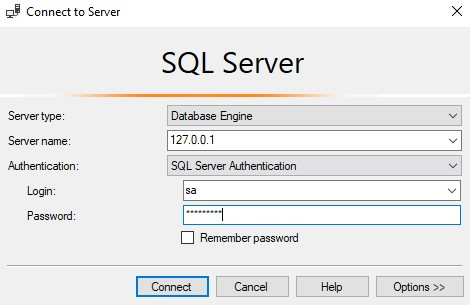
\includegraphics[width=12cm]{./IMAGENES/foto13} 
		\caption{Colocamos el puerto y las credenciales para conectarnos}
	\end{center}
\end{figure}

\begin{figure}[H]
	\begin{center}
		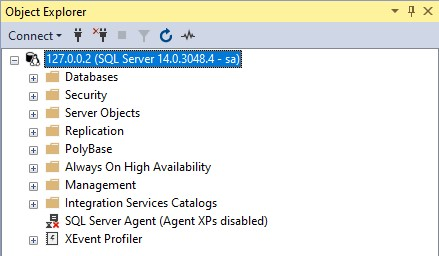
\includegraphics[width=12cm]{./IMAGENES/foto14} 
		\caption{Nos conectamos a la base de datos localhost}
	\end{center}
\end{figure}

\begin{figure}[H]
	\begin{center}
		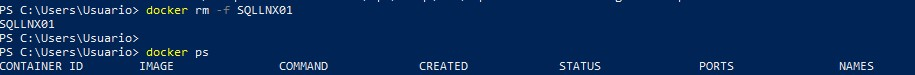
\includegraphics[width=12cm]{./IMAGENES/foto17} 
		\caption{Por último eliminamos nuestra contenedor.}
	\end{center}
\end{figure}


\section{ANALISIS E INTERPRETACION DE RESULTADOS }
\begin{itemize}
	\item ¿Qué indican los resultados? \\
	Pudimos realizar exitosamente la conexión de nuestro contenedor a la base de datos
	\item ¿Que se ha encontrado?\\
	Se ha encontrado una forma rapida y eficiente de trabajar con bases de datos sin la necesidad de instalar el servicio.
\end{itemize}

\section{Actividades Encargadas}
\begin{itemize}
	\item ¿Con qué comando(s) exportaría la imagen de Docker de Microsoft SQL Server a otra PC o servidor? \\
	docker tag 518a41981a6a myRegistry.com/myImage
	docker push myRegistry.com/myImage
	\item ¿Con qué comando(s) podría generar dos volúmenes para un contenedor para distribuir en un volumen el Archivo de Datos (.mdf) y en otro el Archivo Log (.ldf)?\\
	docker volume create ArchivodeDatos.mdf \\
	docker volume create ArchivodeLog.ldf
	\item Genere un nuevo contenedor y cree la base de datos con las siguientes características.\\
	Nombre : FINANCIERA\\
	Archivos : \\
	DATOS (mdf) : Tamaño Inicial : 50MB, Incremento: 10MB, Ilimitado \\
	INDICES (ndf) Tamaño Inicial : 100MB, Incremento: 20MB, Maximo: 1GB \\
	HISTORICO (ndf) Tamaño Inicial : 100MB, Incremento: 50MB, Ilimitado \\
	LOG (ldf) Tamaño Inicial : 10MB, Incremento: 10MB, Ilimitado \\
	¿Cuál sería el script SQL que generaría esta base de datos?
	
	CREATE DATABASE FINANCIERA ON
	PRIMARY(
		Name='Datos',
		FILENAME='C/Program FILES \\Microsoft' SQL Server \\ MSSQL14.MSSQLSERVER\\MSSQL\\DATA\\Datos.mdf',
		SIZE=50MB,
		FILEGROWTH=10MB
	),
	FILEGROUP Indices(
		NAME='Indices',
		FILENAME='C\\Program Files\\Microsoft SQL Server\\MSSQL14.MSSQLSERVER\\MSSQL\\DATA\\indices.ndf',
		SIZE=100MB,
		FILEGROWTH=200,
		MAXSIZE=1GB
	)
	FILEGROUP Indices(
		NAME='Historico',
		FILENAME='C\\Program Files\\Microsoft SQL Server\\MSSQL14.MSSQLSERVER\\MSSQL\\DATA\\Historico.ndf',
		SIZE=100MB,
		FILEGROWTH=200,
		
	)LOG ON(
		NAME='LOGFinanciera',
		FILENAME='C\\Program Files\\Microsoft SQL Server\\MSSQL14.MSSQLSERVER\\MSSQL\\DATA\\LOGFinanciera.ldf',
		SIZE=10MB,
		FILEGROWTH=10MB
);
	
	
\end{itemize}


\section{CONCLUSION}
Los contenedores ayudan a usar bases de datos de forma mas eficiente para poder hacer pruebas o simular ambientes de desarollo o produccion.

\end{document}
